% Created 2018-05-23 Wed 16:08
% Intended LaTeX compiler: pdflatex
\documentclass[12pt]{wx672article}

\usepackage{fullpage}
\usepackage{wx672minted}
\author{Qiyuan Pu(pqy7172@gmail.com)}
\date{\today}
\title{Bypass Guide}
\hypersetup{
 pdfauthor={Qiyuan Pu(pqy7172@gmail.com)},
 pdftitle={Bypass Guide},
 pdfkeywords={},
 pdfsubject={},
 pdfcreator={Emacs 25.2.2 (Org mode 9.1.12)}, 
 pdflang={Cn}}
\begin{document}

\maketitle
\tableofcontents

Please check this webpage as far as possible on the computer, as this webpage currently
does not support the good experience of the mobile phone. Of course, I didn't have much
interest in using web design to make it adapt to the mobile phone. Thank you for your
understanding. :)

Currently this tutorial only provides installation methods for Android and Windows. Of
course my desire is to have a method for all platforms. If your platform is iOS, Mac OS,
etc. please contact me(see bottom), we will continue to complete this document together.
Before I was successfully installed on these platforms, but now I do not have these
platforms so it is not good for screenshots of presentation so need your help in the
future.


If you don't understand anything in the process of reading or operating, or if a link
fails, please email me.

You can reach any corner of the world across the firewall. Have fun. :)

\section*{ATTENTION(Legal Notices)}
\label{sec:org92b9747}
Once you begin to browse this document, you will comply with the following statement I
made. If you not, please stop reading, thanks.
\begin{itemize}
\item The technology that anyone learns from this document CAN ONLY be used for study, work,
scientific research, and entertainment purposes.
\end{itemize}


\begin{itemize}
\item It MUST NOT violate Chinese laws, and MUST NOT intentionally disseminate information
outside of GFW to the mainland of China. It MUST NOT publish excessive remarks. Any
violation of the law is HIS OWN responsibility and HAS NOTHING to do with me.

\item For possible reasons, the techniques described in this document may not achieve the
desired results. The author does not guarantee any of them. Even the authors are not
responsible for solving the problems caused by these operations. However, based on past
experience, what is said here is workable and will not bring any problems.

\item Any individual or group that violates this statement HAS NOTHING to do with me.
\end{itemize}



\section*{Overview}
\label{sec:org2217820}
See bottom for Email address of author. This article is completely a rookie for computers
and mobile phones. As long as you patiently follow the documentation down you can always
visit Google.

Due to some reasons, it is not possible to access and use well-known websites and
applications such as Google and Facebook in mainland China. This article does not intend
to discuss these reasons. My purpose is to enable people to use these services to
facilitate their work, study, life, and entertainment. Everything else has nothing to do
with me. Any problems that come with it are the responsibility of the individual.

For the sake of simplicity, I only discuss how to do it and achieve the desired effect,
not to talk about why. The structure discussed in this article is based on various systems
and hardware platforms. The main hardware platforms include mobile phones and
computers. There are Android and iOS operating systems in the mobile platform. The
computer platform is divided into three systems: Linux, Windows, and Mac. So next I will
follow these classifications to discuss how to achieve the access to Google and other
sites on these platforms.

It is getting harder and harder now to bypass. Now the common practice is to send your
access request to a server first, instead of sending it directly to a Google server. The
intermediate server will visit Google for you and return the result. Well, first of all,
you have to have your own intermediate server. Usually this intermediate server is
available in two ways. The first is to build your own server, and how to build your own
server is a tricky problem. Anyone who reads this document can ask the author how to do
this(see bottom). The other is to buy a server that has already been built by others. Here
I recommend a company that provides this kind of service: \url{https://www.fyzhuji.com}. And if
you decide to buy services provided by the company, I suggest you join the author's
self-built server instead of buying the company provided, so you not only save the trouble
of creating a server, but also avoid spending more to obtain the freedom of information
that you should get. If you think so, please contact the author. In short, I will assume
in this article that you already have a hypothetical server with the following
parameters(of course it doesn't work, you have to have its own available server).

\label{org78958ea}
\begin{itemize}
\item Server Name: 192.168.1.1

\item Remote Port: 8000

\item Password: 123456

\item Encrypt Method: chacha20
\end{itemize}


\section*{Install and Configuration}
\label{sec:org745cbb5}

\subsection*{Mobile Phone}
\label{sec:orga3c3207}
Mobile phones are mainly divided into Android and iOS systems.
\subsubsection*{Android}
\label{sec:org354bc5b}
\begin{itemize}
\item Install
\label{sec:org084bd83}
First we need to install the Android client. Obviously, these clients are hardly available
in mainland China. In my github I provided the software for download: \href{https://github.com/Puqiyuan/Shadowsocks\_Install/blob/master/Shadowsocks.apk}{APK for
Android}. This is open source software, so you shouldn’t worry about security issues such
as back doors.

\item Configuration
\label{sec:orgb98c8c3}
Shadowsocks software runs after the installation is complete. It is probably as shown in
the initial run.

\begin{figure}[!htb]
\centering
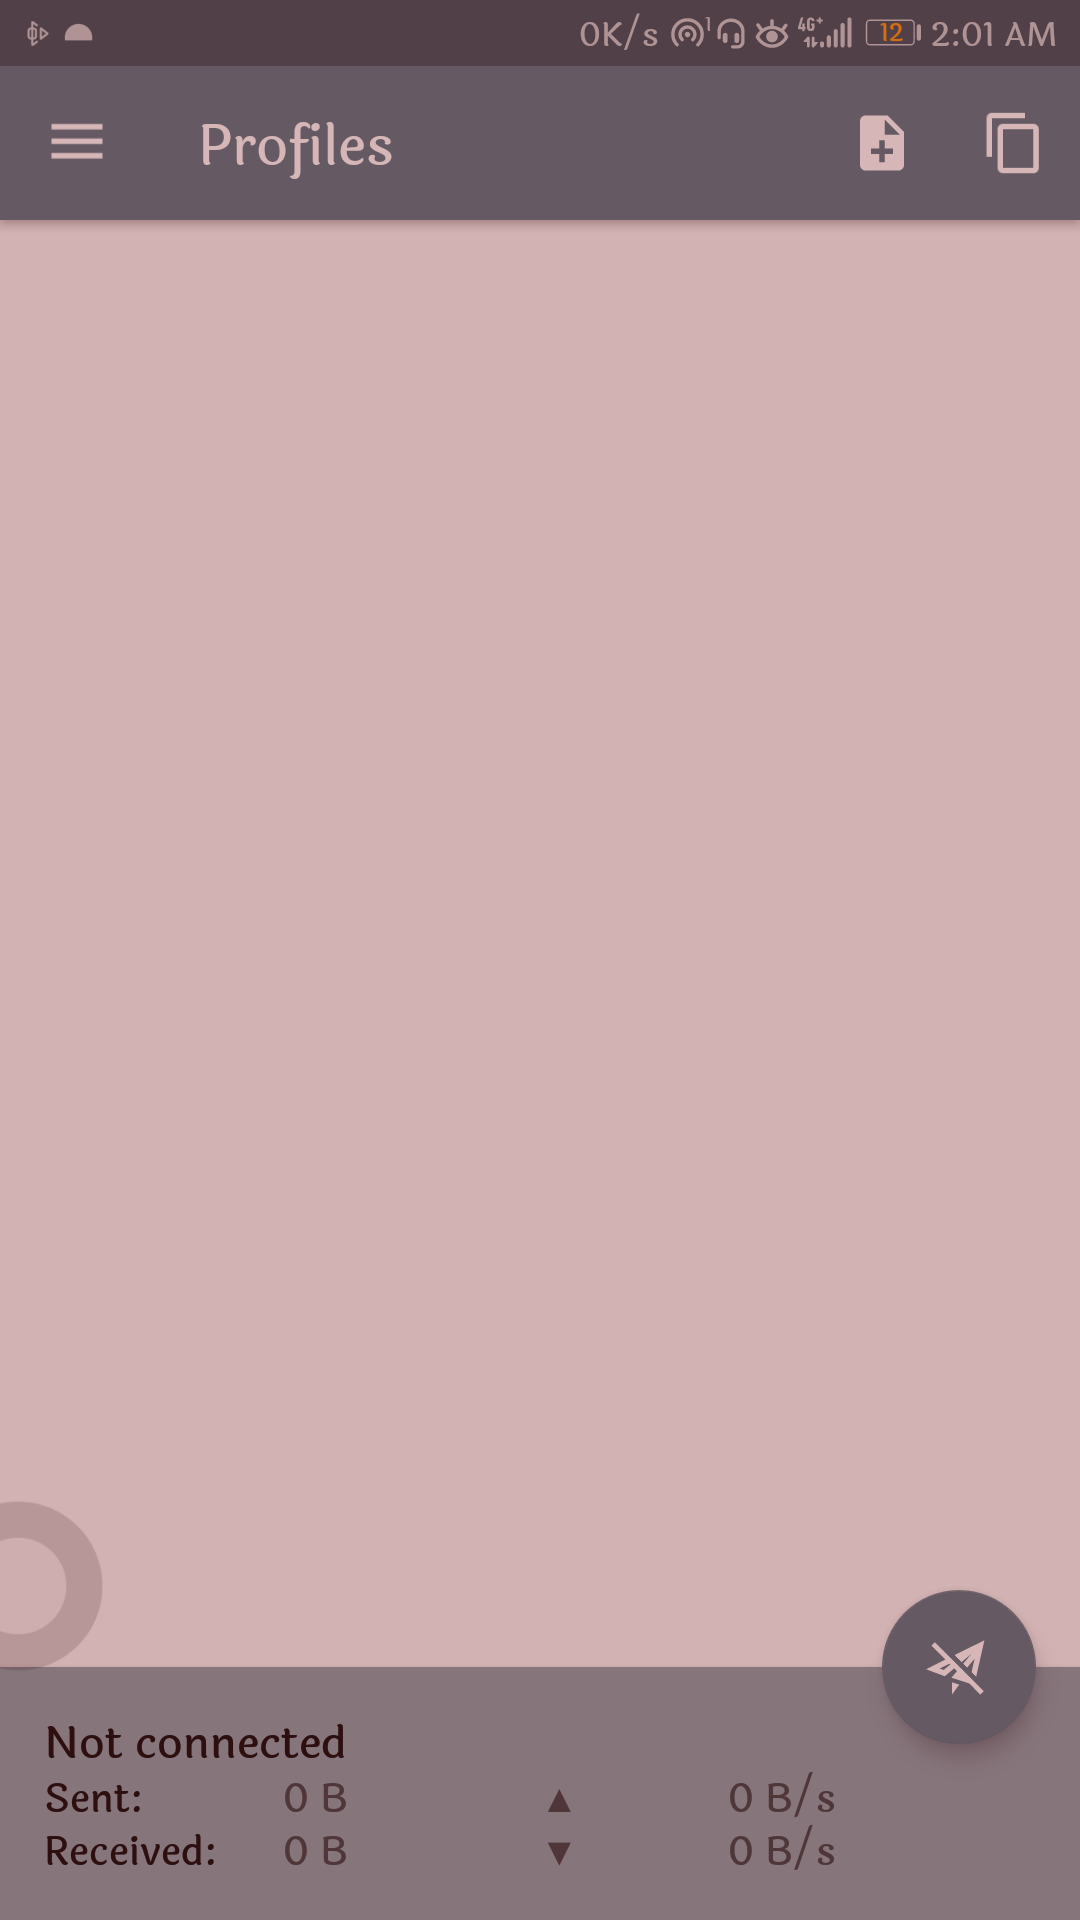
\includegraphics[width=250px]{./images/androidPhone1.jpg}
\caption{\label{fig:orge8c1dfe}
Picture of Shadowsocks initial run}
\end{figure}

Then click the + symbol in the top right corner. After clicking it looks like this:
\begin{figure}[!htb]
\centering
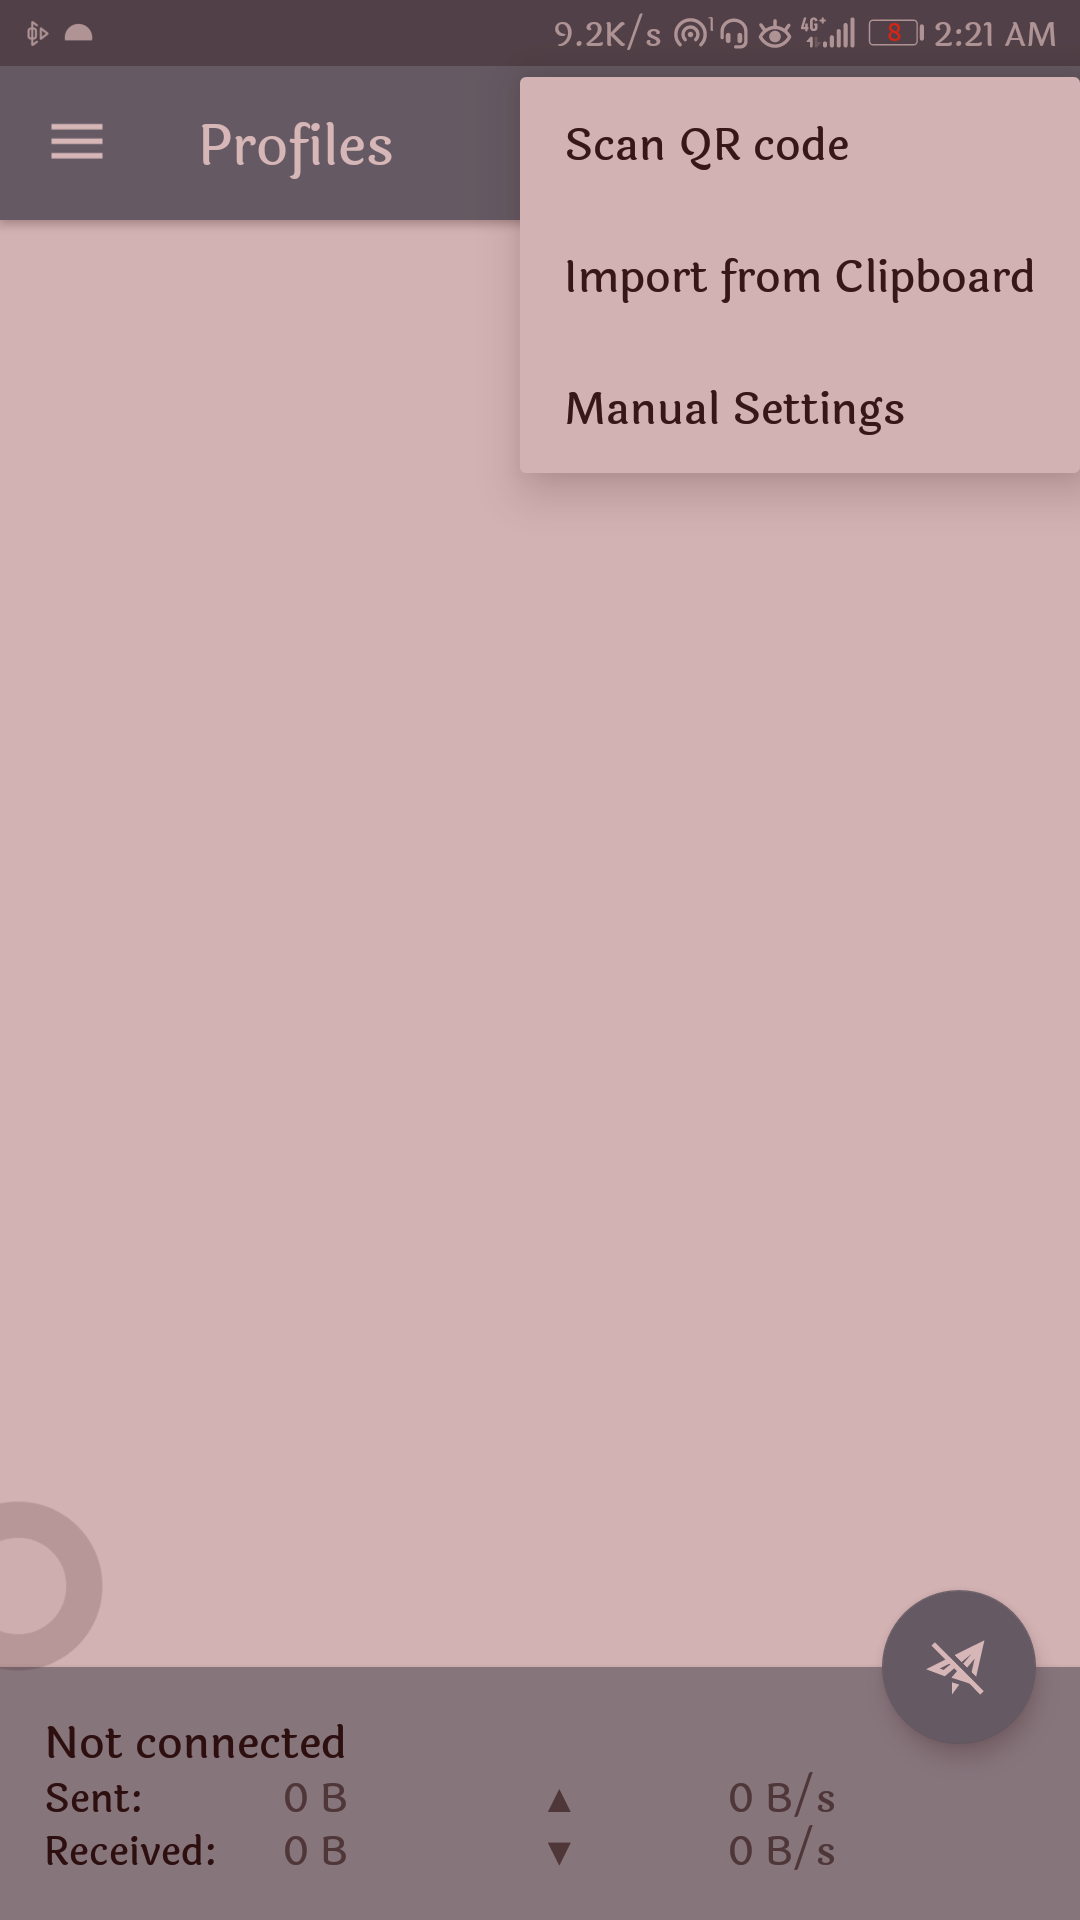
\includegraphics[width=250px]{./images/androidPhone2.jpg}
\caption{\label{fig:orgcd8a967}
Picture of after click + symbol}
\end{figure}

Then click "Manual Settings" in the top right corner. There are three ways to import the
server. Other methods can be tried after you are familiar with this software. After
clicking it looks like this:
\begin{figure}[!htb]
\centering
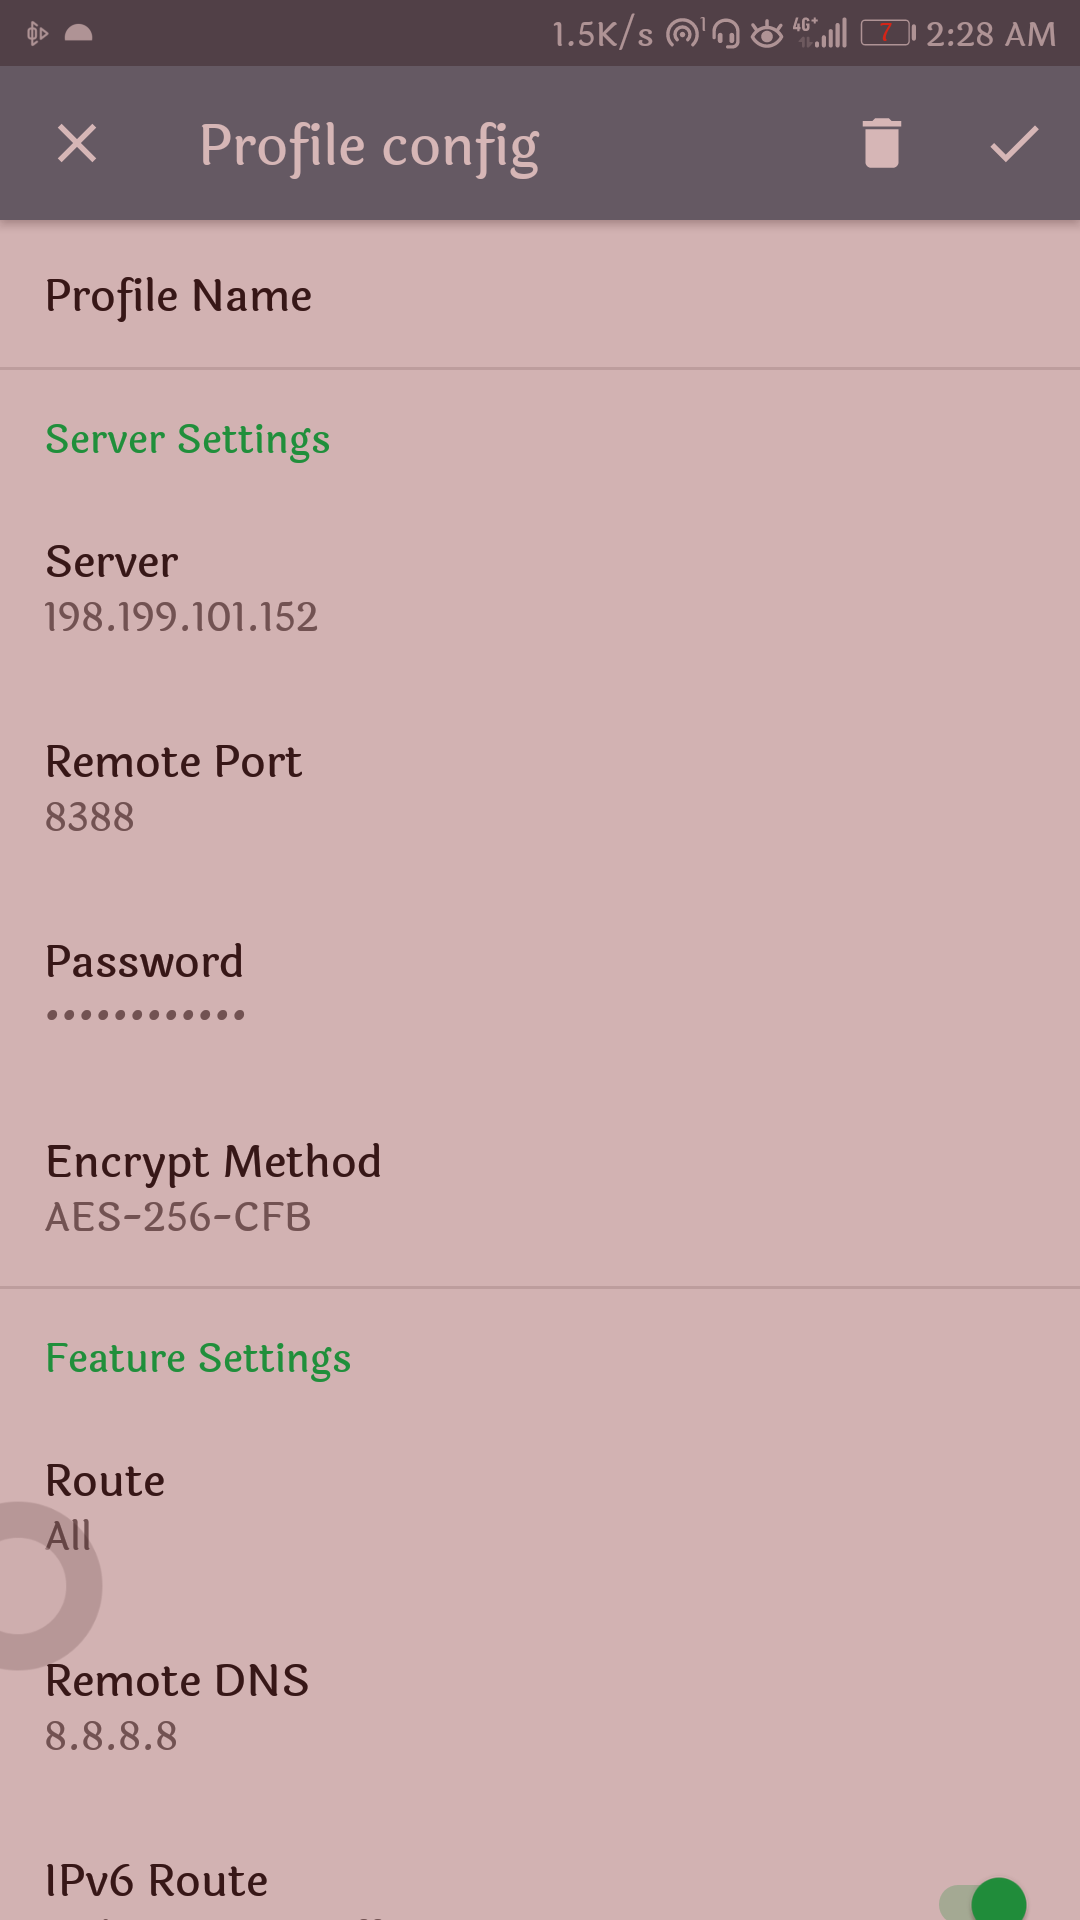
\includegraphics[width=250px]{./images/androidPhone3.jpg}
\caption{\label{fig:org85f908c}
Picture of after click "Manual Setting"}
\end{figure}

Of course, these parameters are not what we assumed \hyperref[org78958ea]{here}. So we must modify it according
to the server parameters assumed \hyperref[org78958ea]{here}. Parameters not mentioned in the screenshot do not
need to be modified. The figure after modifying the parameters is as follows.
\begin{figure}[!htb]
\centering
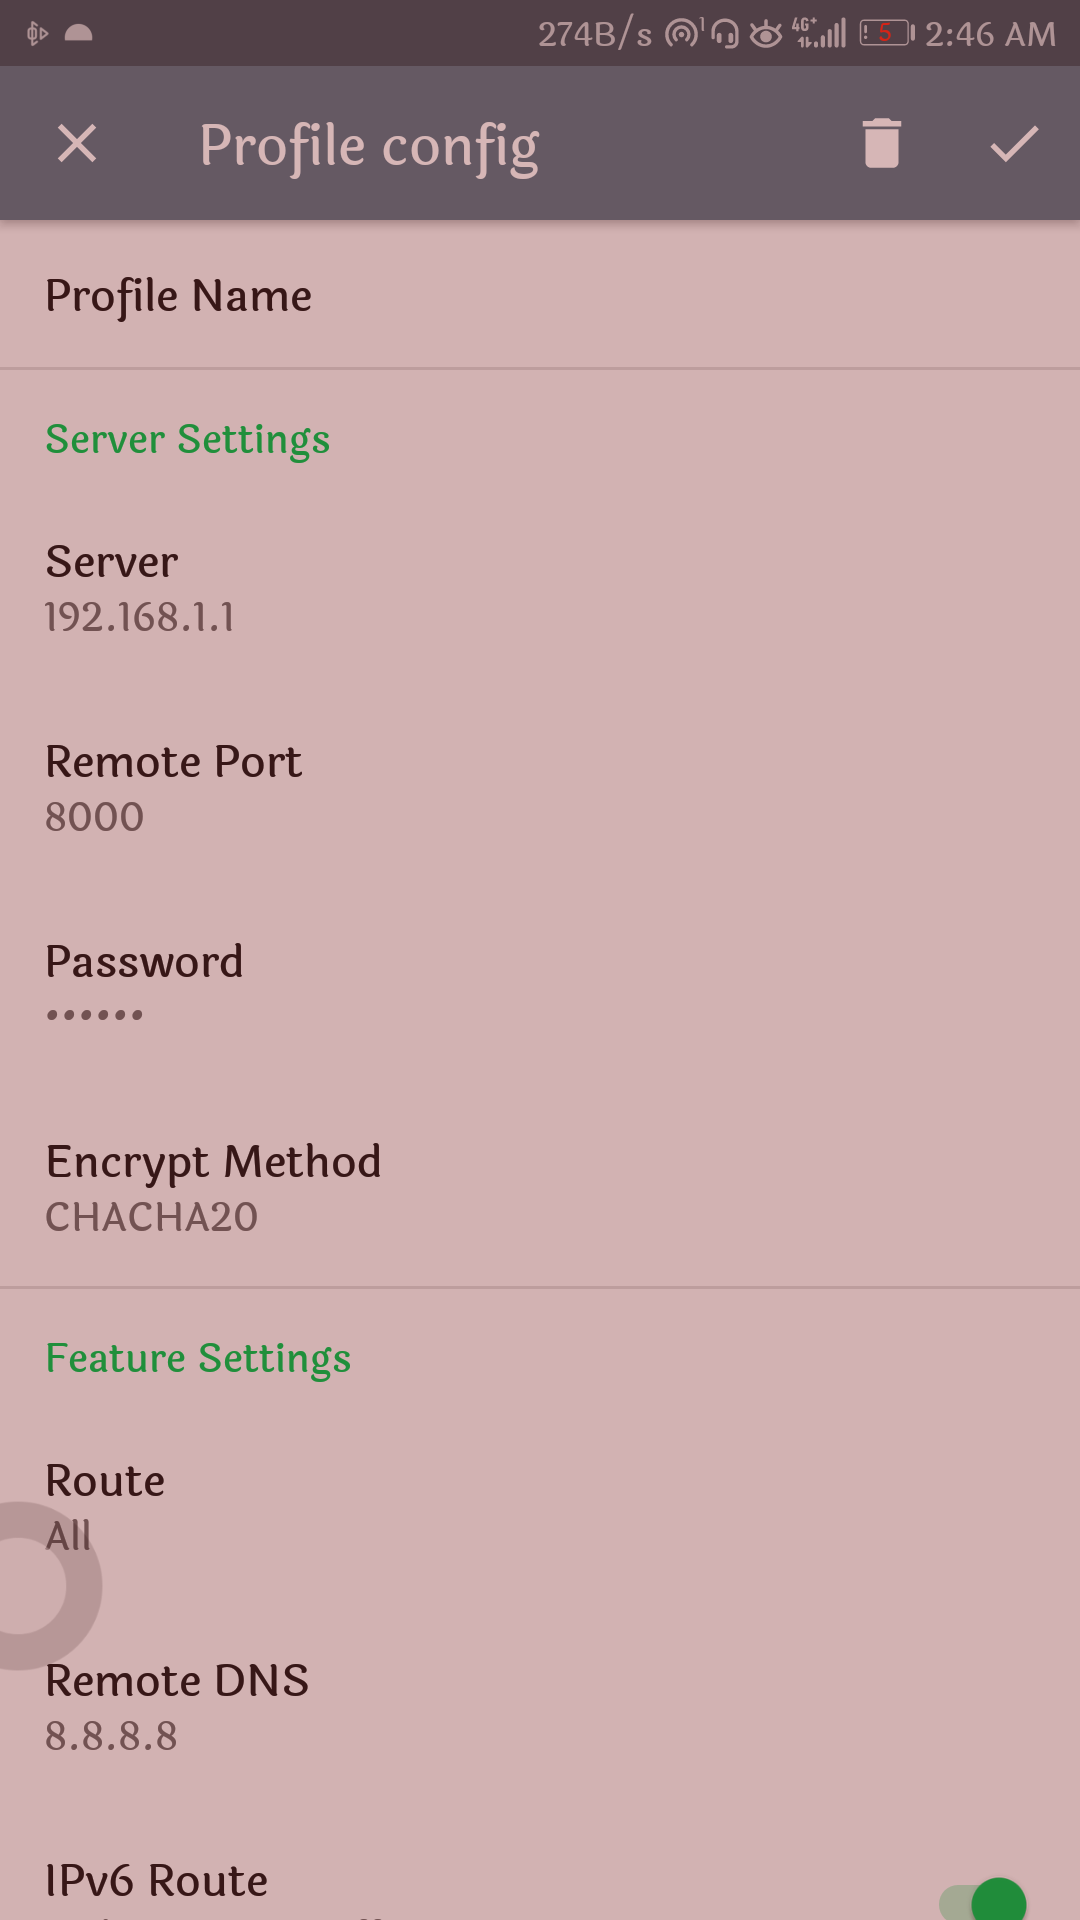
\includegraphics[width=250px]{./images/androidPhone4.jpg}
\caption{\label{fig:org381ae46}
Picture of after modified parameters}
\end{figure}

Then click the small tick in the upper right corner to complete the parameter
configuration. Return to the main interface after completion.
\begin{figure}[!htb]
\centering
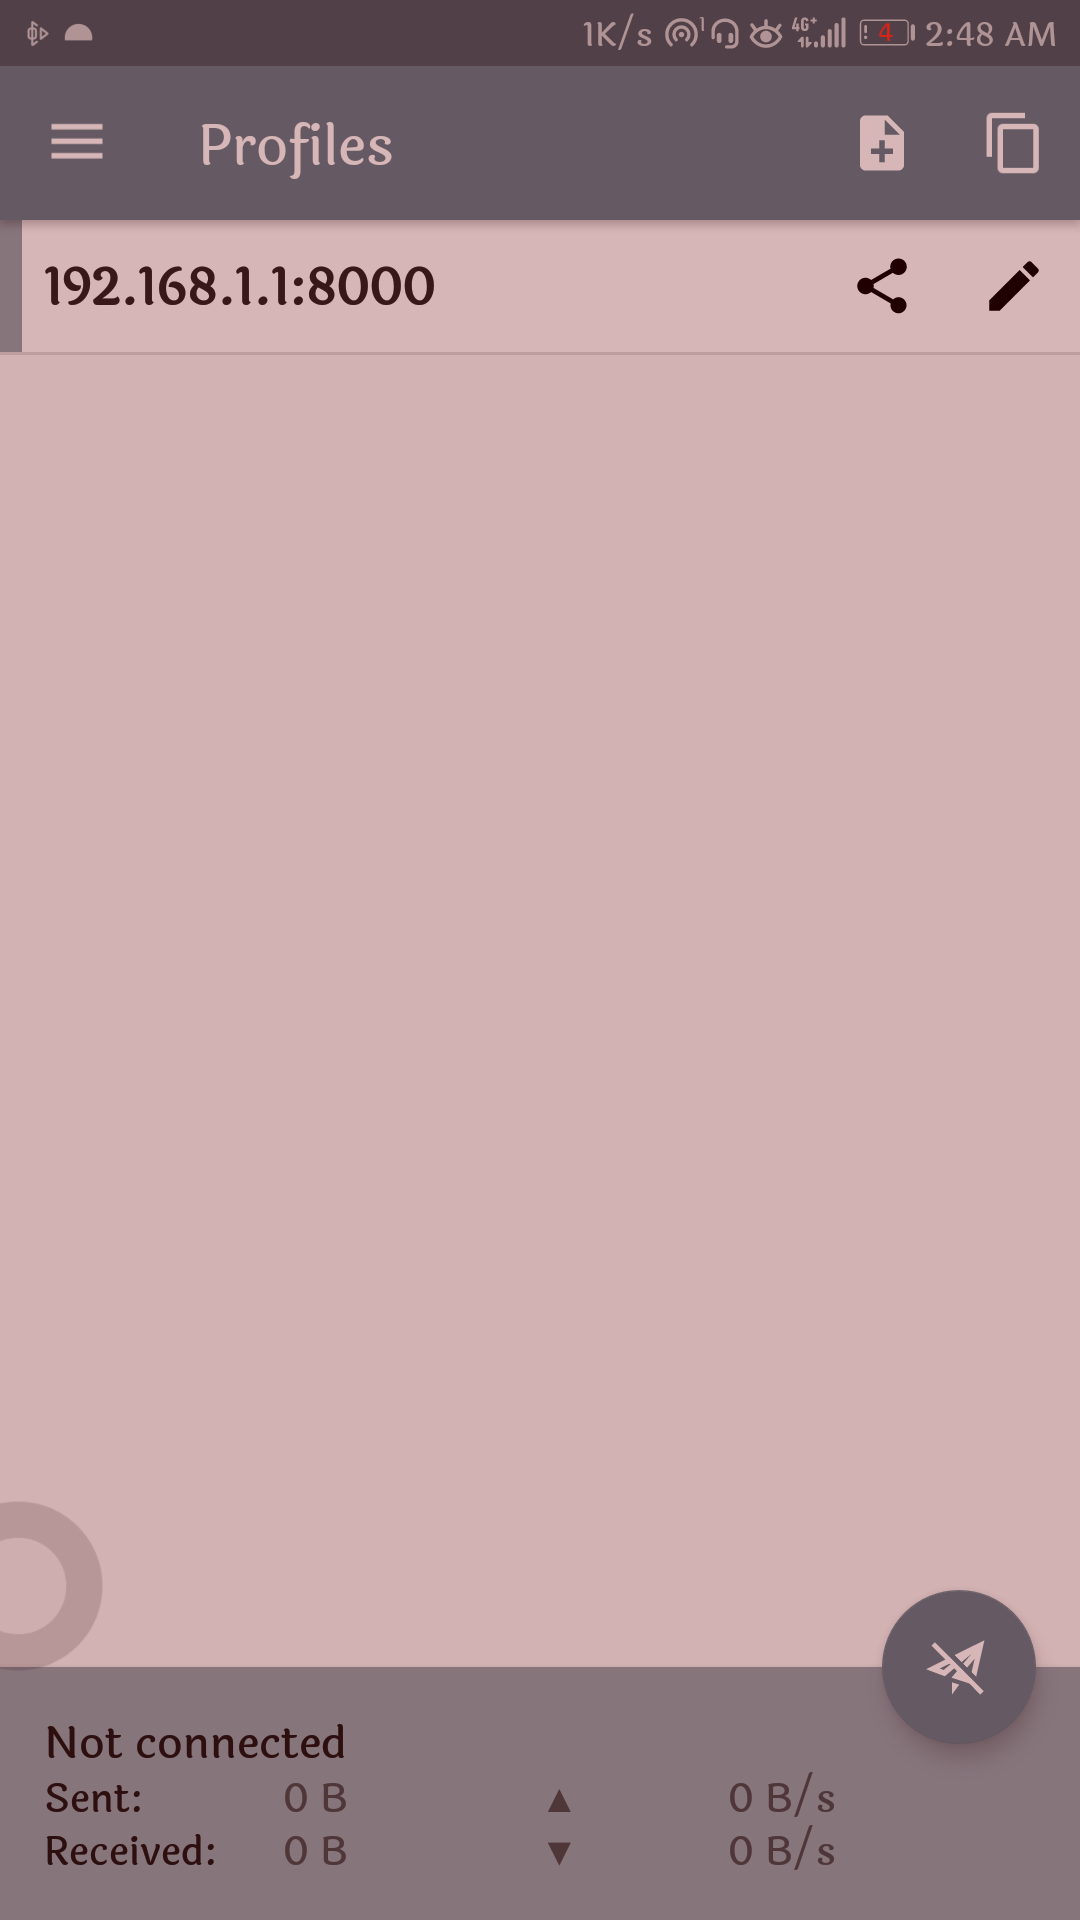
\includegraphics[width=250px]{./images/androidPhone5.jpg}
\caption{\label{fig:orgcae9b03}
Picture of completion of config}
\end{figure}

Then click on the server entry 192.168.1.1. Makes it has a green bar on the left to
achieve the purpose of selecting this server. Like the figure:
\begin{figure}[!htb]
\centering
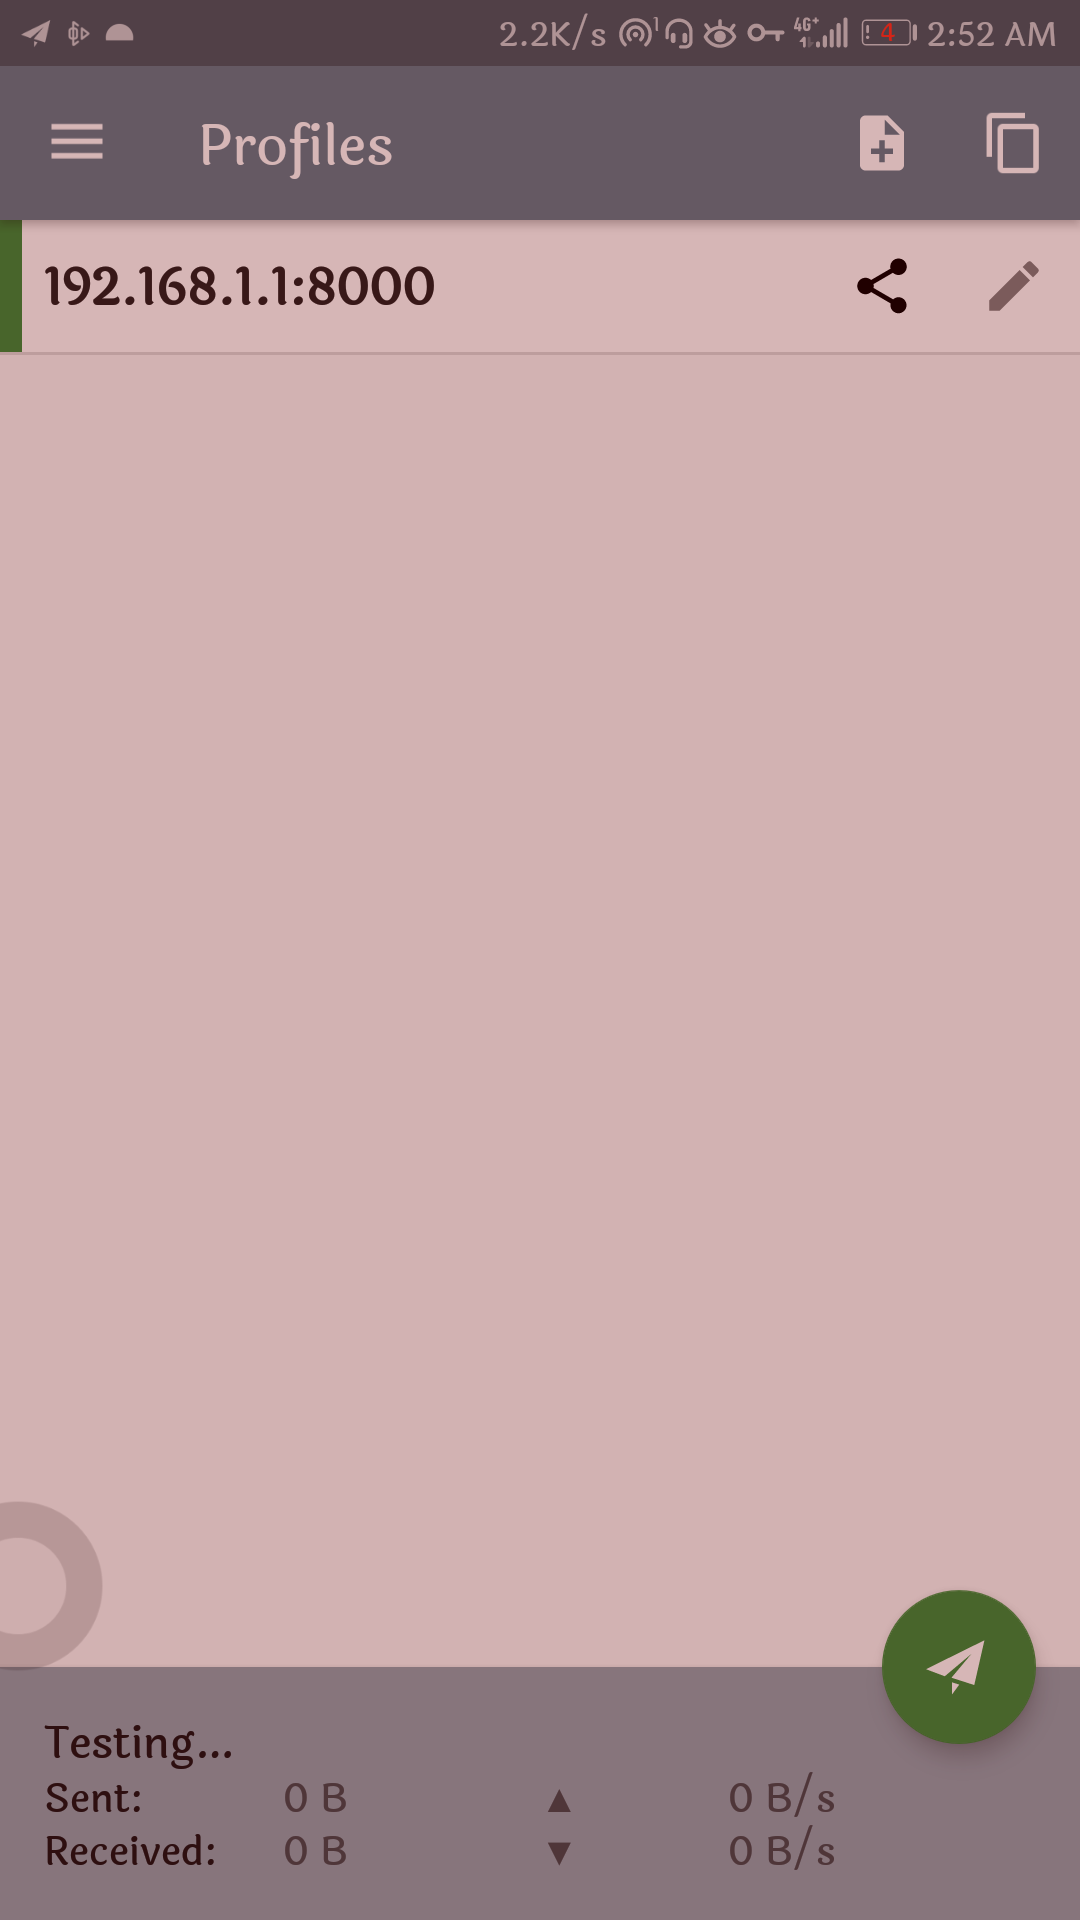
\includegraphics[width=250px]{./images/androidPhone6.jpg}
\caption{\label{fig:org19aa39b}
Picture of running a server}
\end{figure}

Of course, now you can't see the delay. That's because this server is our hypothetical
one. It doesn't work. If it is a normal working server you should see something like this:
\begin{figure}[!htb]
\centering
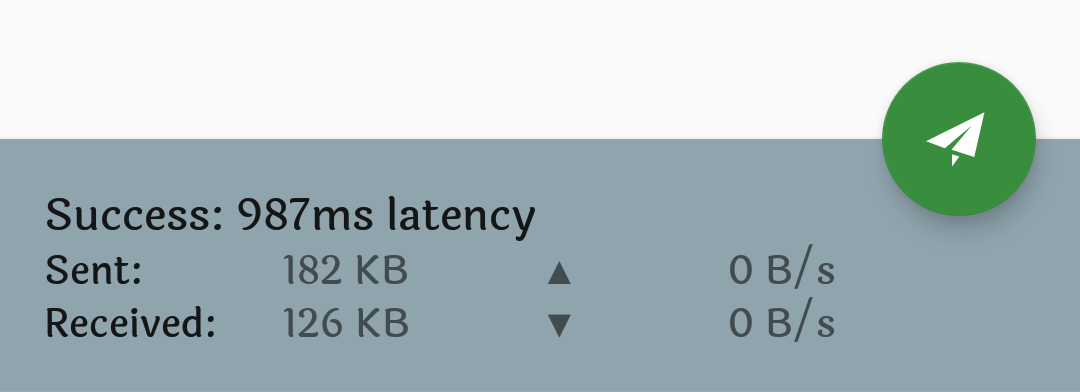
\includegraphics[width=250px]{./images/androidPhone7.jpg}
\caption{\label{fig:org3b18a69}
Picture of running a server in that a working  server}
\end{figure}

If you see a delay like above picture, it means that you have crossed the firewall and now
you can reach anywhere in the world. You can now visit \url{https://www.google.com}. Have
fun. :)
\end{itemize}

\subsection*{Computer}
\label{sec:org482f6e0}
The main computer system is divided into Linux, Windows and Mac OS. Then I installed the
bypass software on these three systems.
\subsubsection*{Windows}
\label{sec:orgdd68f4b}
\begin{itemize}
\item Install
\label{sec:org1340460}
The Windows installation package is in the form of zip. Check \href{https://github.com/shadowsocks/shadowsocks-windows/releases}{here} for download,
like below picture:
\begin{figure}[!htb]
\centering
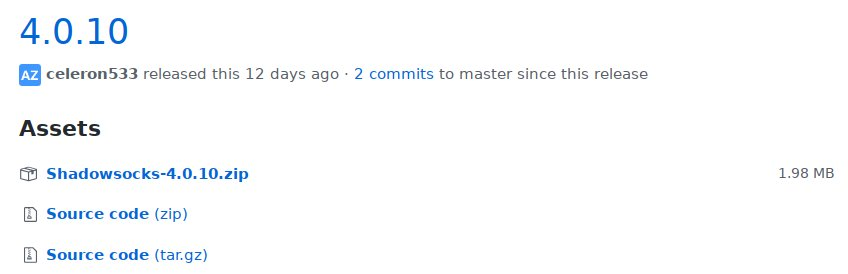
\includegraphics[width=5000px]{./images/windows1.jpg}
\caption{\label{fig:org9210bc0}
Download for Windows install package}
\end{figure}

Click on Shadowsocks-X.X.XX.zip to download and unzip and run. During the initial run, you
may encounter problems with the version of the .Net framework being too low. At this time,
the Windows system will prompt you to upgrade, you only need to follow the prompt to
upgrade. The interface after starting the running is shown below.
\begin{figure}[!htb]
\centering
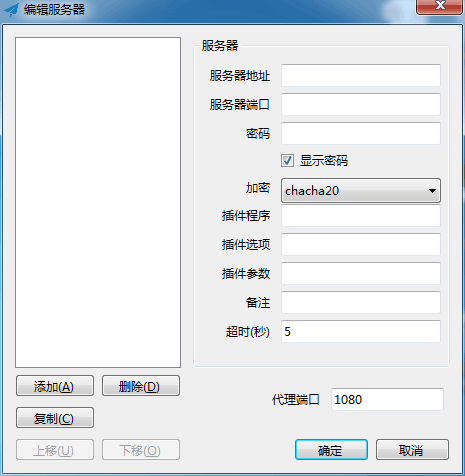
\includegraphics[width=350px]{./images/windows2.jpg}
\caption{\label{fig:orgcdb2573}
Initial running interface}
\end{figure}

Then configure according to the hypothetical server \hyperref[org78958ea]{mentioned} above. Pay attention to
first click on the "添加" before configuration at lower left corner. Last click "确定".


\begin{figure}[!htb]
\centering
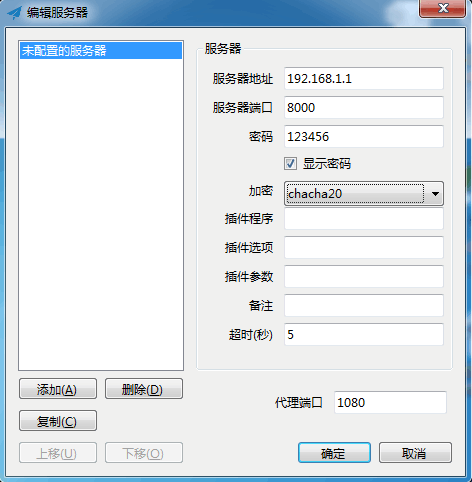
\includegraphics[width=350xp]{./images/windows3.jpg}
\caption{\label{fig:org0a5ee01}
Complete the configuration}
\end{figure}

After completion, there will be a small aircraft symbol in the lower right corner of the
screen. Click it and configure it as shown in the figure below.
\begin{figure}[!htb]
\centering
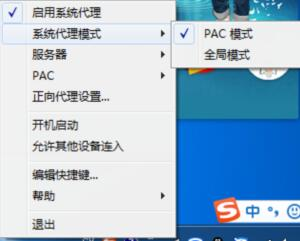
\includegraphics[width=350xp]{./images/windows4.jpg}
\caption{\label{fig:org4a74505}
Enable proxy in PAC mode}
\end{figure}

You can now visit \url{https://www.google.com}.
\end{itemize}
\end{document}